\documentclass[11pt]{article}
\usepackage[sc]{mathpazo} %Like Palatino with extensive math support
\usepackage{fullpage}
\usepackage[authoryear,sectionbib,sort]{natbib}
\linespread{1.7}
\usepackage[utf8]{inputenc}
\usepackage{lineno}
\usepackage{titlesec}
% Added later
\usepackage{amsmath}  % for equations
\usepackage{graphicx} % for figures

\titleformat{\section}[block]{\Large\bfseries\filcenter}{\thesection}{1em}{}
\titleformat{\subsection}[block]{\Large\itshape\filcenter}{\thesubsection}{1em}{}
\titleformat{\subsubsection}[block]{\large\itshape}{\thesubsubsection}{1em}{}
\titleformat{\paragraph}[runin]{\itshape}{\theparagraph}{1em}{}[. ]\renewcommand{\refname}{Literature Cited}

%%%%%%%%%%%%%%%%%%%%%
% Line numbering
%%%%%%%%%%%%%%%%%%%%%
%
% Please use line numbering with your initial submission and
% subsequent revisions. After acceptance, please turn line numbering
% off by adding percent signs to the lines %\usepackage{lineno} and
% to %\linenumbers{} and %\modulolinenumbers[1] below.
%
% To avoid line numbering being thrown off around math environments,
% the math environments have to be wrapped using
% \begin{linenomath*} and \end{linenomath*}
%
% (Thanks to Vlastimil Krivan for pointing this out to us!)

\title{Template and Guidelines for Using \LaTeX{} in \textit{The~American~Naturalist} }

% This version of the LaTeX template was last updated on
% July 16, 2024.

%%%%%%%%%%%%%%%%%%%%%
% Authorship
%%%%%%%%%%%%%%%%%%%%%
% Please commet out authorship information while your paper is under review. 
% You will need to add this information back in to your final files after
% acceptance.

\author{Owen E. Cook$^{1,\ast}$ \\ 
Generic H. Collaborator$^{2,\dag}$ \\ 
Additional Q. Expert$^{3}$}

\date{}

\begin{document}

\maketitle

\noindent{} 1. University of Chicago, Chicago, Illinois 60637;

\noindent{} 2. University of Toronto, Toronto, Ontario M5S 1A5, Canada;

\noindent{} 3. Middle Eastern Technical University, Çankaya, Ankara 06800, Turkey.

\noindent{} $\ast$ Corresponding author; e-mail: amnat@uchicago.edu.

\noindent{} $\dag$ Deceased.

\bigskip

\textit{Manuscript elements}: Figure~1, figure~2, table~1, appendix~A (for print; including figure~A1, figure~A2, and table~A1), supplemental PDF. Figure~2 is to print in color.

\bigskip

\textit{Keywords}: Examples, model, template, guidelines.

\bigskip

\textit{Manuscript type}: Article. %Or note, natural history miscellany note, comment, reply, invited symposium, featured topic, or historical perspective.

\bigskip

\noindent{\footnotesize Prepared using the suggested \LaTeX{} template for \textit{Am.\ Nat.}}

\linenumbers{}
\modulolinenumbers[1]

\newpage{}

\section*{Abstract}

Lorem ipsum dolor sit amet, consectetur adipiscing elit. Sed non risus. Suspendisse lectus tortor, dignissim sit amet, adipiscing nec, ultricies sed, dolor. Cras elementum ultrices diam. Praesent quis dolor in dolor molestie cursus et ac nisi. Vestibulum ante purus, semper eget est vitae, vehicula ornare nisl. Morbi efficitur euismod enim, nec feugiat tellus cursus eget. 

\newpage{}

\section*{Introduction}

% The journal does not have numbered sections in the main portion of
% articles. Please refrain from using section references (à la
% section~\ref{section:CountingOwlEggs}), and refer to sections by name
% (e.g. section ``Counting Owl Eggs'').

Start with major transition in evolution. What to say about this??? fraternal transition and egalitarian transition (estrela 2016)
\section*{Methods}

\begin{figure}[ht]
	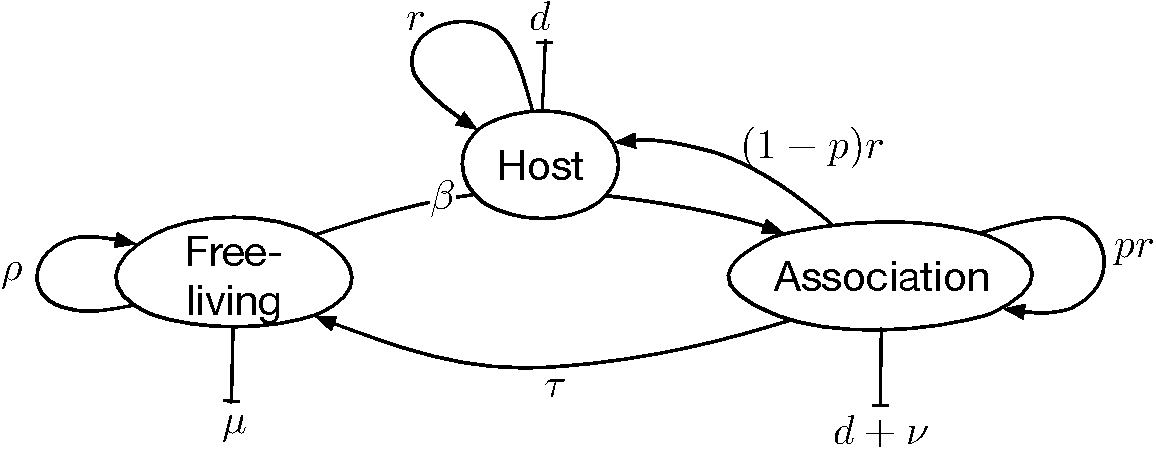
\includegraphics[width=\linewidth]{model_sketch}
	\caption{Model sketch}
	\label{Fig:model_sketch}
\end{figure}

\begin{align}
	\frac{dF}{dt}     & = \rho F +\tau A - \alpha F^2 - \mu F - \beta H F \\
	\frac{dA}{dt}    & = \beta H F +  p r A - \gamma (A + H) A - (\nu + d)  A \\
	\frac{dH}{dt}    & = r (1 - p) A + r  H -\beta H F   - \gamma (A + H) H - d H 
\end{align}

\subsection*{Second-order heading}

Lorem ipsum nulla facilisi, pace \citet{LemKapEx07}. Etiam semper, orci sit amet facilisis interdum, tellus nunc consequat erat, quis viverra nisi diam ut metus. Pellentesque cursus, sapien malesuada euismod iaculis, mauris purus interdum diam, vel vestibulum justo enim vitae tellus. Nunc interdum lorem sit amet diam volutpat tristique. Quisque pulvinar ac metus commodo lacinia (\citealt{Ing11,Xiao2015}).  

\subsubsection*{Third-order heading}

Usually two or three levels of heading will be all you need. Journal style even permits a fourth level in case you need it.

\paragraph*{Fourth-order heading}
The quick red fox jumps over the lazy brown dog in this paragraph as well. Donec mauris nibh, volutpat vehicula viverra at, iaculis congue sem. Praesent eget erat rhoncus erat sollicitudin volutpat. 

\begin{equation}
{ \frac{1}{N_k-1} \sum \limits_{t=1}^{N_k} (M_{tjk} - \bar{M}_{jk})^2}
\end{equation}

Praesent quis dolor in dolor molestie cursus et ac nisi. Vestibulum ante purus, semper eget est vitae, vehicula ornare nisl. Morbi efficitur euismod enim, nec feugiat tellus cursus eget. Donec mauris nibh, volutpat vehicula viverra at, iaculis congue sem.

\subsection*{Another second-order heading}

As \citet{Xiao2015} argued, phasellus porttitor eros et ante condimentum, eget facilisis orci condimentum. Nulla facilisi. Proin placerat elit blandit, euismod dolor nec, dapibus diam. Mauris posuere malesuada lacus, at elementum lacus auctor eu (fig~\ref{Fig:Jumps}A). 

\section*{Results}

Lorem ipsum dolor sit amet. Aenean pulvinar malesuada commodo (see \citealt{DavisEtAl2011}; table~\ref{Table:Founders}). Sed aliquet mauris odio, in tristique dui egestas a. Etiam eu malesuada quam. Suspendisse tincidunt eu erat sit amet vulputate. Duis at arcu et nisl dictum mattis. Maecenas vel cursus ante. Cras eleifend elit nec velit sollicitudin fermentum in ac mauris. Pellentesque rutrum magna vel elit maximus hendrerit. 

\subsection*{The height of the jump}

Aenean eu pellentesque quam (fig.~\ref{Fig:OkapiHorn}). Nam pellentesque augue eu finibus lacinia. Nullam nec justo vitae odio imperdiet rhoncus vitae vitae quam. Pellentesque porttitor metus et lectus ornare, ac cursus urna efficitur (fig~\ref{Fig:Jumps}B). 

\subsection*{The laziness of the dog}

Example paragraph with embedded references (video~\ref{VideoExample}, fig.~\ref{Fig:AnotherFigure}). 
If you have deposited data to Dryad, it is advisable to cite them somewhere in the main text (usually in the Methods or Results sections). A sentence like the following will do: All data are available in the Dryad Digital Repository (\citealt{CookEtAl2015}).

\section*{Discussion}

Nam pulvinar lorem at lorem ultrices, vel accumsan massa feugiat (\citealt{Ing11}). Proin tristique velit eget lacus iaculis, in pellentesque nulla varius. Phasellus sodales est odio, eu pulvinar magna pellentesque eu. Sed ut lobortis eros. Aliquam eget metus turpis. Sed et convallis lectus, id tincidunt enim. In porta nibh ut lacus feugiat, non consequat orci rhoncus. Morbi blandit at augue nec tempor. Sed fringilla ipsum ut justo viverra, ut euismod nisi gravida.

Curabitur non posuere augue, id suscipit orci. Nunc luctus accumsan aliquam. Cras egestas turpis vitae nisl vulputate interdum. Donec pellentesque libero egestas tortor pharetra laoreet. Phasellus facilisis auctor ligula, eu sollicitudin mi sagittis non.

\section*{Conclusion}

Duis pharetra enim at libero cursus, eu commodo mi vestibulum. Nullam eget velit nec lectus viverra sodales. Suspendisse egestas, eros at dictum tincidunt, mi orci laoreet libero, eget rutrum sapien arcu blandit odio.

%%%%%%%%%%%%%%%%%%%%%
% Acknowledgments
%%%%%%%%%%%%%%%%%%%%%
% You may wish to remove the Acknowledgments section while your paper 
% is under review as the Acknowledgments may reveal your identity.
% If you remove this section, you will need to add it back in to your
% final files after acceptance.

\section*{Acknowledgments}

OEC would like to thank Madlen Wilmes, Gyuri Barab\'{a}s, Flo D\'{e}barre, Vlastimil K\v{r}ivan, and Greg Dwyer for their comments and suggestions on this template.

%%%%%%%%%%%%%%%%%%%%%
% Statement of Authorship
%%%%%%%%%%%%%%%%%%%%%
% This section should also be commented out while your MS is undergoing
% double-blind review. The specifics should of course be adapted to
% your paper, but the paragraph below gives some hints of possible
% contributions.

\section*{Statement of Authorship}

OEC conceived the experiments, collected the data, and wrote the original draft.
GHC provided specimens and analyzed the model.
AQE oversaw data analysis and developed the code. 
All authors reviewed and edited the writing at all stages of revision.

\section*{Data and Code Availability}

On initial submission, you may use this section to provide a URL for editors and reviewers that is `private for peer review'. After acceptance, this section must be updated with correct, working DOIs for data and code deposits (such as in Zenodo, Dryad, or DataVerse). An example statement could resemble the following: All data and code for this work are available from the Dryad Digital Repository, \citealt{CookEtAl2015}). 

\section*{Appendix A: Additional Methods and Parameters}

% In most cases, authors should typeset supplementary material in a separate,
% author-supplied PDF. For author-supplied PDFs, please consult the
% AmNat_supp_template.tex document, available from
% https://www.journals.uchicago.edu/journals/an/instruct 
%
% If you want to use cross-references within the supplemental TeX file,
% it may be helpful to \usepackage{xr} and include the command 
% \externaldocument{name-of-supplemental-tex-file}
%
% The Appendix instructions below apply to cases in which
% a brief appendix is to appear in print after the main body of the article.
% That notably includes descriptions of methods, tables defining parameters,
% and other material necessary for reproducing the MS's results.
%
% Please reset counters for the appendix (thus normally figure A1, 
% figure A2, table A1, etc.).
%
% Most AmNat articles have no more than one print appendix. If your article
% has more than one, counters for each appendix should match the letter of
% that appendix. For example, tables in Appendix B should be numbered table B1, % table C2, etc. This applies to tables, equations, and figures.
%
% It's better not to use the \appendix command, because we have some
% formatting peculiarities that \appendix conflicts with.

\renewcommand{\theequation}{A\arabic{equation}}
% redefine the command that creates the equation number.
\renewcommand{\thetable}{A\arabic{table}}
\setcounter{equation}{0}  % reset counter 
\setcounter{figure}{0}
\setcounter{table}{0}

\subsection*{Fox--dog encounters through the ages}

The quick red fox jumps over the lazy brown dog. The quick red fox has always jumped over the lazy brown dog. The quick red fox began jumping over the lazy brown dog in the 19th century and has never ceased from so jumping, as we shall see in figure~\ref{Fig:Jumps}. But there can be surprises (figure~\ref{Fig:JumpsOk}).

If the order and location of figures is not otherwise clear, feel free to include explanatory dummy text like this:

[Figure A1 goes here.]

[Figure A2 goes here.]

\subsection*{Further insights}

Tables in the appendices can appear in the appendix text (see table~\ref{Table:Rivers} for an example), unlike appendix figure legends which should be grouped at the end of the document together with the other figure legends.

\begin{table}[h]
\caption{Various rivers, cities, and animals}
\label{Table:Rivers}
\centering
\begin{tabular}{lll}\hline
River        & City        & Animal            \\ \hline
Chicago      & Chicago     & Raccoon           \\
Des Plaines  & Joliet      & Coyote            \\
Illinois     & Peoria      & Cardinal          \\
Kankakee     & Bourbonnais & White-tailed deer \\
Mississippi  & Galena      & Bald eagle        \\ \hline
\end{tabular}
\bigskip{}
\\
{\footnotesize Note: See table~\ref{Table:Founders} below for further table formatting hints.}
\end{table}

Lorem ipsum dolor sit amet, as we have seen in figures~\ref{Fig:Jumps} and \ref{Fig:JumpsOk}.


%%%%%%%%%%%%%%%%%%%%%
% Bibliography
%%%%%%%%%%%%%%%%%%%%%
% You can either type your references following the examples below, or
% compile your BiBTeX database and paste the contents of your .bbl file
% here. The amnatnat.bst style file should work for this---but please
% let us know if you run into any hitches with it!
%
% If you upload a .bib file with your submission, please upload the .bbl
% file as well; this will be required for typesetting.
%
% The list below includes sample journal articles, book chapters, and
% Dryad references.

\begin{thebibliography}{}

\bibitem[{Cook et~al.(2015)Cook, Collaborator, and Expert}]{CookEtAl2015}
Cook, O.~E., G.~H. Collaborator, and A.~Q. Expert. 2015.
\newblock Data from: Template and guidelines for using \LaTeX{} in \textit{The American Naturalist}.
\newblock American Naturalist, Dryad Digital Repository, https://dx.doi.org/10.5061/dryad.XYZAB123.

\bibitem[{Darwin(1859)Darwin}]{OriginSpec}
Darwin, C. 1859.
\newblock On the origin of species by means of natural selection, or the preservation of favoured races in the struggle for life.
\newblock J.~Murray, London.

\bibitem[{Davis et~al.(2011)Davis, Brakora, and Lee}]{DavisEtAl2011}
Davis, E.~B., K.~A. Brakora, and A.~H. Lee. 2011.
\newblock Evolution of ruminant headgear: a review.
\newblock Proceedings of the Royal Society~B 278:2857--2865.

\bibitem[{Inglis et~al.(2011)Inglis, Roberts, Gardner, and Buckling}]{Ing11}
Inglis, R.~F., P.~G. Roberts, A.~Gardner, and A.~Buckling. 2011.
\newblock Spite and the scale of competition in \textit{Pseudomonas
  aeruginosa}.
\newblock American Naturalist 178:276--285.

\bibitem[{Fastovsky(2009)Fastovsky}]{LemKapEx07}
Fastovsky, D.~E. 2009.
\newblock Ideas in dinosaur paleontology: resonating to social and political context.
\newblock Pages 239--253 \emph{in} D. Sepkoski and M. Ruse, eds. The Paleobiological Revolution. University of Chicago Press, Chicago~IL.

\bibitem[{Xiao et~al.(2015)Xiao, McGlinn, and White}]{Xiao2015}
Xiao, X., D.~J. McGlinn, and E.~P. White. 2015.
\newblock A strong test of the maximum entropy theory of ecology.
\newblock American Naturalist 185:E705--E80.

\section*{References Cited Only in the Online Enhancements}

% This section is for works cited in your supplemental PDF but
% not in the main text.

\bibitem[{Tytler(1759)Tytler}]{tytler-mqos}
Tytler, W. 1759.
\newblock The Inquiry, Historical and Critical, into the Evidence against Mary Queen of Scots, and an Examination of the Histories of Dr. Robertson and David Hume with respect to that Evidence.
\newblock W.~Creech, Edinburgh.

\end{thebibliography}

\newpage{}

\section*{Tables}
\renewcommand{\thetable}{\arabic{table}}
\setcounter{table}{0}

\begin{table}[h]
\caption{Founders of \textit{The~American Naturalist}}
\label{Table:Founders}
\centering
\begin{tabular}{lll}\hline
Early editor            & Years with the journal \\ \hline
Alpheus S. Packard Jr.  & 1867--1886 \\
Frederick W. Putnam     & 1867--1874 \\ 
Edward S. Morse         & 1867--1871 \\ 
Alpheus Hyatt           & 1867--1871 \\
Edward Drinker Cope$^a$ & 1878--1897 \\
J.~S. Kingsley          & 1887--1896 \\ \hline 
\end{tabular}
\bigskip{}
\\
{\footnotesize Note: Table titles should be short. Further details should go in a `notes' area after the tabular environment, like this. $^a$ Published the first description of \textit{Dimetrodon}.}
\end{table}

\newpage{}

\section*{Figure legends}

\begin{figure}[h!]
%\includegraphics{horn-of-okapi}
\caption{Figure legends can be longer than the titles of tables. However, they should not be excessively long---in most cases, they should be no more than 100 words each.}
\label{Fig:OkapiHorn}
\end{figure}



\begin{figure}[h!]
%\includegraphics{elegance}
\caption{In this way, figure legends can be listed at the end of the document, with references that work, even though the graphic itself should be included for final files after acceptance. Instead, upload the relevant figure files separately to Editorial Manager; Editorial Manager should insert them at the end of the PDF automatically.}
\label{Fig:AnotherFigure}
\end{figure}

% Figure legends for any print appendices you might have.

\renewcommand{\thefigure}{A\arabic{figure}}
\setcounter{figure}{0}

\begin{figure}[h!]
%\includegraphics{jumps20m}
\caption{\textit{A}, the quick red fox proceeding to jump 20~m straight into the air over not one, but several lazy dogs. \textit{B}, the quick red fox landing gracefully despite the skepticism of naysayers.}
\label{Fig:Jumps}
\end{figure}

\begin{figure}[h!]
%\includegraphics{jumps20m}
\caption{The quicker the red fox jumps, the likelier it is to land near an okapi. For further details, see \citet{LemKapEx07}.}
\label{Fig:JumpsOk}
\end{figure}


%%%%%%%%%%%%%%%%%%%%%
% Videos
%%%%%%%%%%%%%%%%%%%%%
% If you have videos, journal style for them is generally similar to that for
% figures. 

%%%%% Include the text below if you have videos

\renewcommand{\figurename}{Video} 
\renewcommand{\thefigure}{S\arabic{figure}}
\setcounter{figure}{0}

\begin{figure}[h!]
%\includegraphics{VideoScreengrab.jpg}
\caption{Video legends can follow the same principles as figure legends. Counters should be set and reset so that videos and figures are enumerated separately.}
\label{VideoExample}
\end{figure}

\renewcommand{\figurename}{Figure}
\setcounter{figure}{1}

%%%%% Include the above if you have videos


\end{document}
